 \documentclass[a4paper,12pt]{article}
 \usepackage{float}
 \usepackage{hyperref}
 \usepackage{graphicx}
 \graphicspath{ {images/} }
 
 \usepackage{listings}
 \title{Final report}
 \author{The Waypointers}
 
 \begin{document}
 	
 	\section{Design}
 	The design of this Traffic simulator is divided in 3 parts. Those three parts are:
 	\begin{itemize}
 		\item GUI
 		\item Common
 		\item Simulation
 	\end{itemize}
 	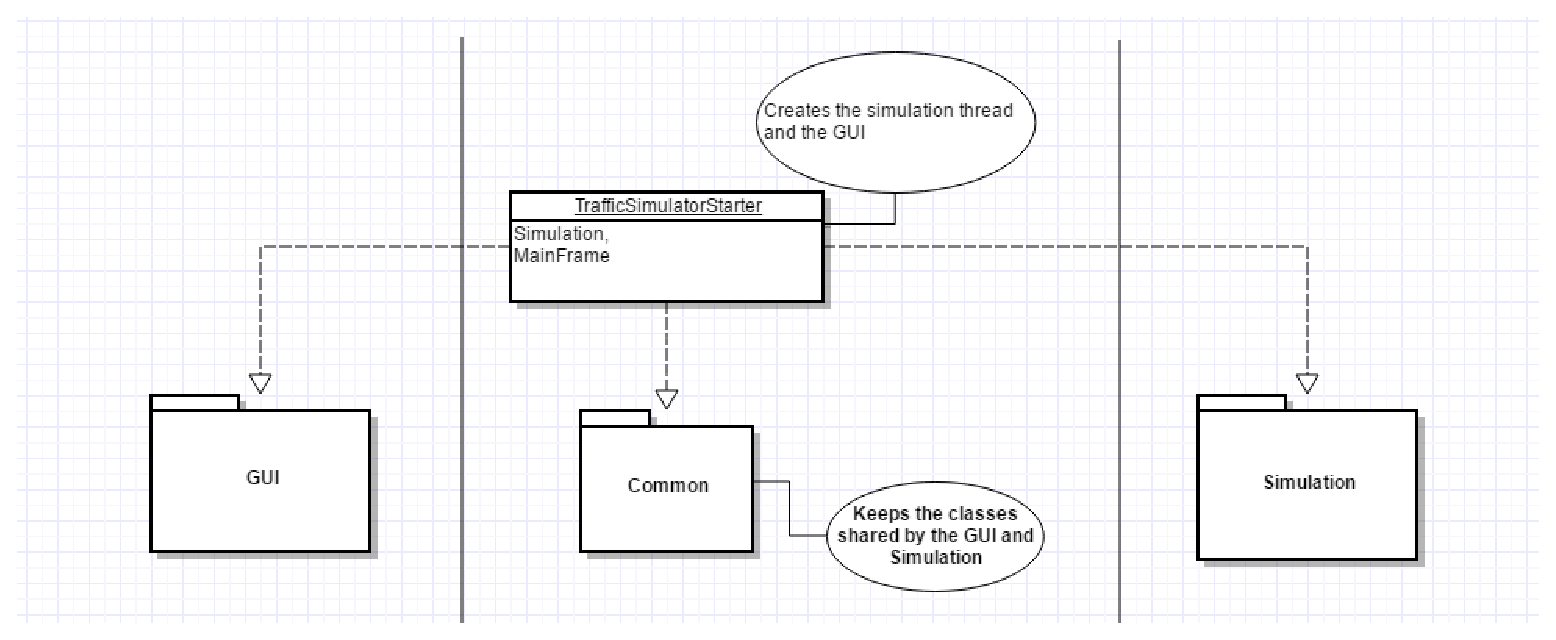
\includegraphics[scale=0.6]{designIMG}
 	
 	\subsection{about}
 	The Simulation part is the core of the traffic simulator, where the actual computing and decisions of vehicles happen. Common is shared by both Simulation and GUI, it contains classes that are used by both other parts of the Traffic simulator. GUI is where the graphics are drawn and shown to the user, it is the part of the Traffic simulator the user interacts with.
 	\newline
 	We decided to go with this design, because we concluded that it would be the easiest if the Simulation part where the computing happens is completely separated from the GUI part. This way it was simpler for us to work on the project and to divide the work between group members.
 	\subsection{"WorldState"}
 	The only object that the both GUI and Simulation see is the “WorldState” object. The” WorldState” object represent the current state of the Traffic simulator. The Simulation builds the “WorldState” object from the values it computes and then the GUI uses the information and draws the graphics.
 	\subsection{Vehicles}
 	All Vehicles inside Simulation are represented as an interface “IVehicle”, because they share many identical methods that need to be implemented in different ways depending on the vehicle type. But because the GUI doesn’t need all these information we decided to pass a different object to the GUI, an object from common “VehicleDTO”. This object is a much simpler version of the vehicle that contains only the necessary information to draw the vehicle on the correct location.
 	
 \end{document}